\chapter{Lecture 18: Schwarz-Christoffel Mappings}

\begin{example}
    Find the Schwarz-Christoffel mapping from $\mathbb{H} = \{z \in \mathbb{C} : \Im(z) > 0\}$ to
    $$w_1 = 0 \qquad w_0 = \sigma_0 + i\tau_0\qquad \sigma_0 < 0, \tau_0 > 0$$
    \begin{figure}[H]
        \centering
        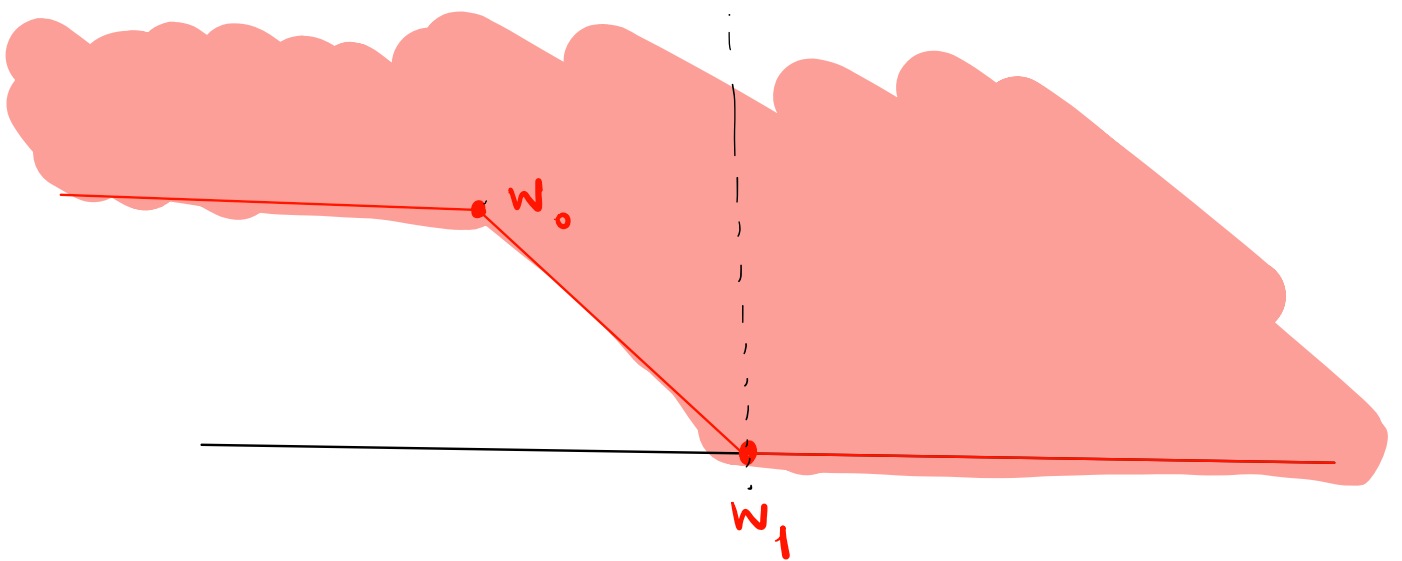
\includegraphics[width=0.5\textwidth]{LECTURE_18/graph.png}
        \caption{Graph}
    \end{figure}
    \begin{align}
        \theta_0 = \arctan(\frac{\tau_0}{\sigma_0}) \in (-\pi, 0), \quad \theta_1 = -\theta_0
    \end{align}
    We choose the points $x_0 = -1, x_1 = 1$ as the pre-image vertices. Now we write:
    \begin{align}
        f'(z) & = A (z + 1)^{-\frac{\theta_0}\pi} (z - 1)^{\frac{\theta_0}\pi}
    \end{align}
    This gives us our general form of $f'(z)$, which can't be integrated easily. So let's take a specific angle  where $\sigma_0 = 0 \rightarrow \theta_0 = -\frac{\pi}{2}$.
    \begin{figure}[H]
        \centering
        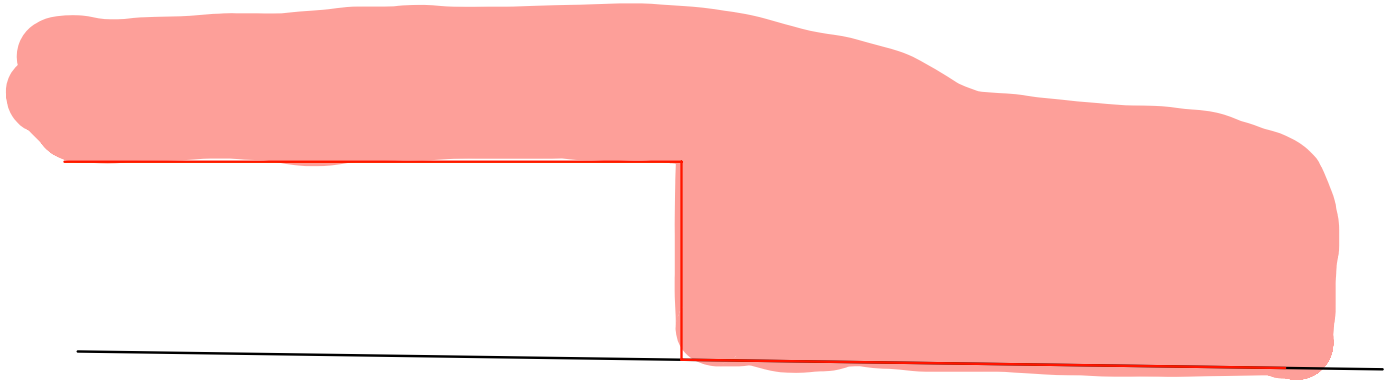
\includegraphics[width=0.5\textwidth]{LECTURE_18/graph1.png}
        \caption{Graph}
    \end{figure}
    \begin{align}
        f'(z) & = A \left(\frac{z + 1}{z - 1}\right)^{\frac{1}{2}}                                                      \\
        f'(z) & = A\left(\frac{z + 1}{z - 1}\frac{z + 1}{z + 1}\right)^{\frac{1}{2}}                                    \\
        f'(z) & = A\frac{z + 1}{(z^2 - 1)^{\frac{1}{2}}}                                                                \\
        f(z)  & = A\int \frac{z + 1}{(z^2 - 1)^{\frac{1}{2}}}dz + B                                                     \\
        f(z)  & = A\left(\int \frac{z}{(z^2 - 1)^{\frac{1}{2}}}dz + \int \frac{1}{(z^2 - 1)^{\frac{1}{2}}}dz\right) + B \\
        f(z)  & = A\left((z^2 -1)^\frac{1}2+ \text{Log}(z+ (z^2 -1)^\frac{1}2)\right) + B                               \\
    \end{align}
    Now we can find use the pre-image vertices to find $A$ and $B$. First we map $x_0 = -1$ to $w_0 = i\tau_0$:
    \begin{align}
        f(-1) & = w_0 = i\tau_0 = A\left((1 -1)^\frac{1}2+ \text{Log}(-1+ (1 -1)^\frac{1}2)\right) + B \\
              & = A(\text{Log}(-1)) + B                                                                \\
              & = A(i\pi) + B
    \end{align}
    \begin{align*}
        f(1) & = w_1 = 0 = A\left((1 -1)^\frac{1}2+ \text{Log}(1+ (1 -1)^\frac{1}2)\right) + B \\
             & = A(\text{Log}(1)) + B                                                          \\
             & = B
    \end{align*}
    This gives us $B = 0$ and $A = \frac{\tau_0}{\pi}$. So our final mapping is:
\end{example}

\begin{example}
    Find the Schwarz-Christoffel mapping from $\mathbb{H} = \{z \in \mathbb{C} : \Im(z) > 0\}$ to
    \begin{figure}[H]
        \centering
        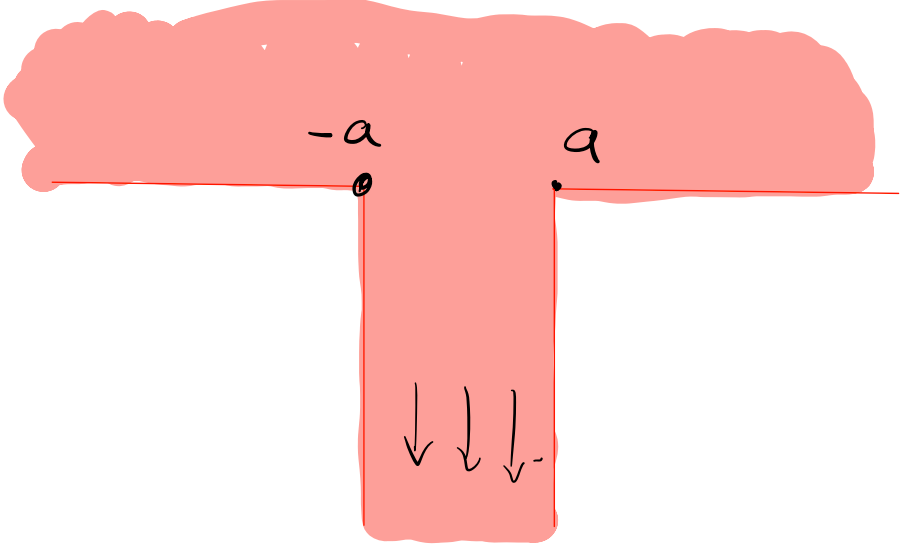
\includegraphics[width=0.5\textwidth]{LECTURE_18/graph2.png}
        \caption{Graph}
    \end{figure}
    \begin{align}
        a > 0, a \in \mathbb{R}
    \end{align}
    \textbf{Idea:} Let's approximate the valley with a triangle extending infinitely downwards
    \begin{figure}[H]
        \centering
        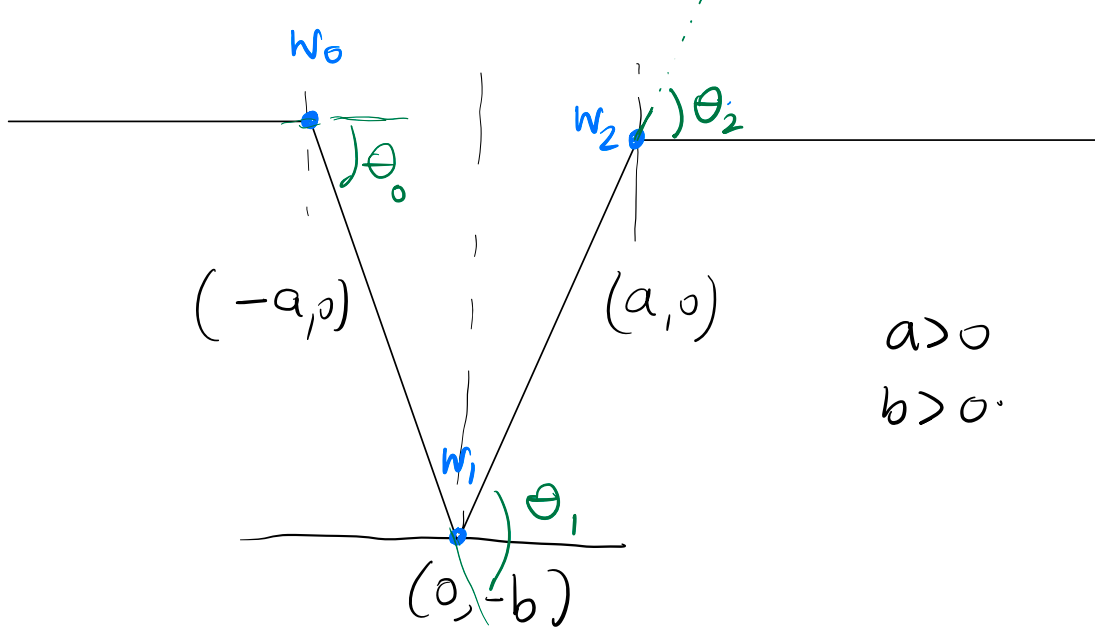
\includegraphics[width=0.5\textwidth]{LECTURE_18/graph3.png}
        \caption{Graph}
    \end{figure}
    We take the limit as $b \rightarrow \infty$. Then we can approximate the angles as:
    \begin{align}
        \theta_0 & = \arctan (\frac{-b}{a}) \approx \frac{-\pi}{2}                  \\
        \theta_2 & = - \arctan(\frac{b}{a}) \approx \frac{-\pi}{2}                  \\
        \theta_1 & = 0 \quad \text{triangles can only have angles that sum to } \pi
    \end{align}
    We choose the points $x_0 = -1, x_1 = 1$ as the pre-image vertices. Now we write:
    \begin{align}
        f'(z) & = A (z + 1)^{-\frac{-\theta_0}\pi}z^{\frac{-\theta_1}\pi} (z - 1)^{\frac{-\theta_2}\pi} \\
        f'(z) & = A (z + 1)^{\frac{1}{2}}z^{-1} (z - 1)^{\frac{1}{2}}                                   \\
    \end{align}
    Thus:
    \begin{align}
        f'(z) & = A\left(\frac{z^2 - 1}{z^2}\right)^{\frac{1}{2}}          \\
              & = A \sqrt{1 - \frac{1}{z^2}}                               \\
        f(z)  & = A\int \sqrt{1 - \frac{1}{z^2}}dz + B
              & = A \left(\sqrt{z^2 - 1} + \arcsin(\frac{1}{z})\right) + B
    \end{align}
    Don't worry about how the integration was done, if you're asked to do it on the exam, you're fucked. Now we can find use the pre-image vertices to find $A$ and $B$. First we map $x_0 = -1$ to $w_0 = -a$:
    \begin{align}
        f(-1) & = w_0 = -a = A \left(\sqrt{1 - 1} + \arcsin(-1)\right) + B \\
        -a    & = A \left(\arcsin(-1)\right) + B                           \\
        -a    & = A \left(-\frac{\pi}{2}\right) + B
    \end{align}
    Now we map $x_1 = 1$ to $w_1 = a$:
    \begin{align}
        f(1) & = w_1 = a = A \left(\sqrt{1 - 1} + \arcsin(1)\right) + B \\
        a    & = A \left(\arcsin(1)\right) + B                          \\
        a    & = A \left(\frac{\pi}{2}\right) + B
    \end{align}
    This gives us $B = 0$ and $A = \frac{2a}{\pi}$. So our final mapping is:
    \begin{align}
        f(z) = \frac{2a}{\pi} \left(\sqrt{z^2 - 1} + \arcsin(\frac{1}{z})\right)
    \end{align}
\end{example}

\begin{example}
    Find the Schwarz-Christoffel mapping from $\mathbb{H}/\{it \in \mathbb{C} : 0 \leq t \leq a\}$ to $\mathbb{H} = \{z \in \mathbb{C} : \Im(z) > 0\}$
    \begin{figure}[H]
        \centering
        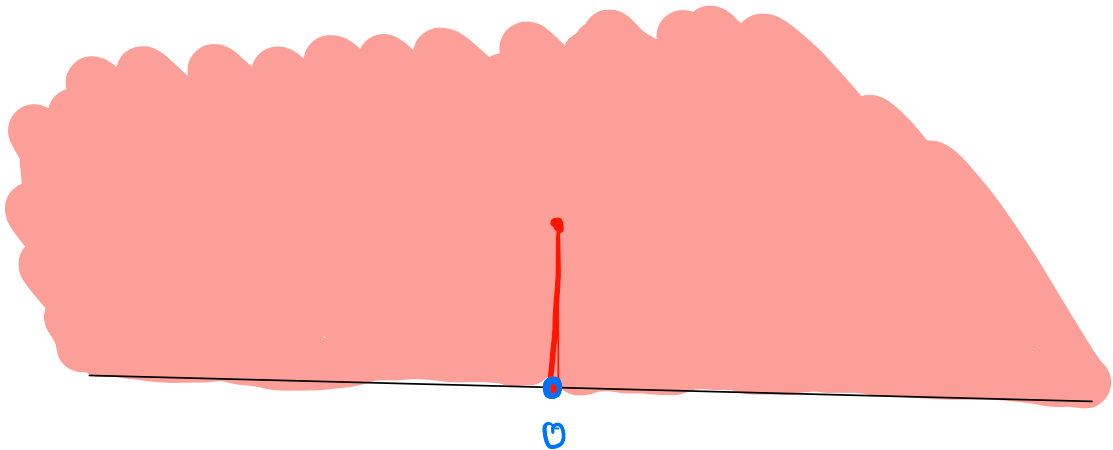
\includegraphics[width=0.5\textwidth]{LECTURE_18/graph4.png}
        \caption{Image Mapping}
    \end{figure}
    We can observe the image vertices to be $w_0 = -\epsilon, w_1 = ia, w_2 = \epsilon$ where $\epsilon \to 0$.
    First, let's view this as the limit of the following domain:
    \begin{figure}[H]
        \centering
        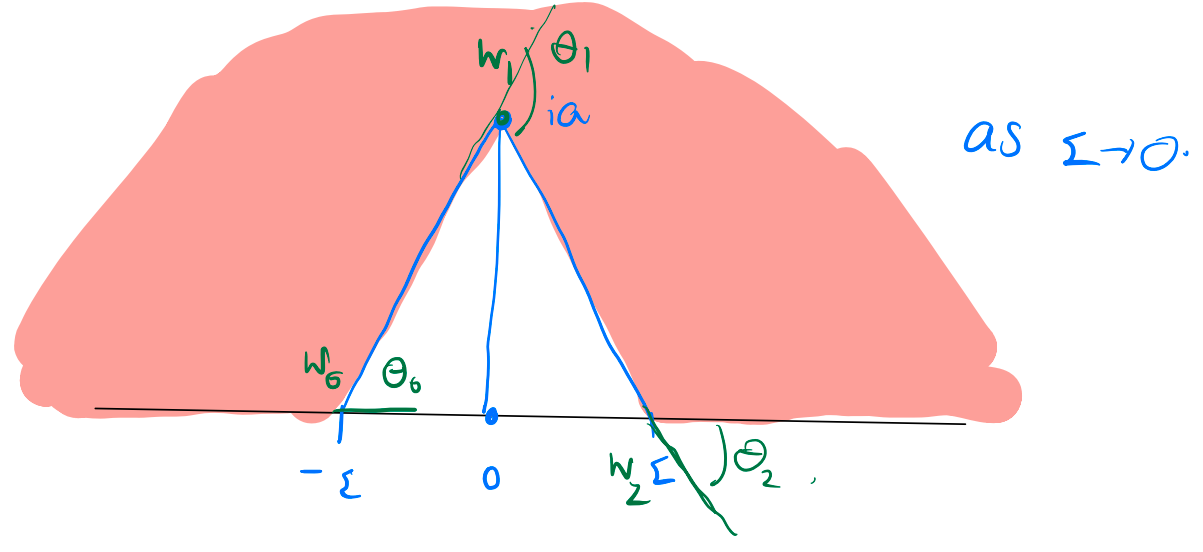
\includegraphics[width=0.5\textwidth]{LECTURE_18/graph5.png}
        \caption{Domain as the limit of a triangle}
    \end{figure}
    Then we can say that the angles are:
    \begin{align}
        \theta_0 & = \frac{\pi}{2} \\
        \theta_1 & = -\pi          \\
        \theta_2 & = \frac{\pi}{2}
    \end{align}
    We choose the points $x_0 = -1, x_1 = 0, x_2 = 1$ as the pre-image vertices. Now we write:
    \begin{align}
        f'(z) & = A (z + 1)^{\frac{-1}{2}}z(z - 1)^{\frac{-1}{2}} \\
              & = A \frac{z}{\sqrt{z^2 - 1}}                      \\
        f(z)  & = A \int \frac{z}{\sqrt{z^2 - 1}}dz + B           \\
              & = A(\sqrt{z^2 - 1}) + B
    \end{align}
    Now we can find use the pre-image vertices to find $A$ and $B$. First we map $x_0 = -1$ to $w_0 = 0$:
    \begin{align}
        f(-1) = w_0 = 0 & = A(\sqrt{1 - 1}) + B \\
        0               & = B                   \\
        f(0) = w_1 = ia & = A(\sqrt{0 - 1})     \\
        A = a                                   \\
    \end{align}
    This gives us $B = 0$ and $A = a$. So our final mapping is:
    \begin{align}
        f(z) = a\sqrt{z^2 - 1}
    \end{align}
\end{example}